\begin{exercises}
\item Finding limits of convergent sequences can be a challenge. However, there is a useful tool we can adapt from our study of limits of continuous functions at infinity to use to find limits of sequences. We illustrate in this exercise with the example of the sequence
    \[\frac{\ln(n)}{n}.\]
    \ba
    \item Calculate the first 10 terms of this sequence. Based on these calculations, do you think the sequence converges or diverges? Why?

    \item For this sequence, there is a corresponding continuous function $f$ defined by
    \[f(x) = \frac{\ln(x)}{x}.\]
    Draw the graph of $f(x)$ on the interval $[0,10]$ and then plot the entries of the sequence on the graph. What conclusion do you think we can draw about the sequence $\left\{\frac{\ln(n)}{n}\right\}$ if $\lim_{x \to \infty} f(x) = L$? Explain.

    \item Note that $f(x)$ has the indeterminate form $\frac{\infty}{\infty}$ as $x$ goes to infinity. What idea from differential calculus can we use to calculate $\lim_{x \to \infty} f(x)$? Use this method to find $\lim_{x \to \infty} f(x)$. What, then, is $\lim_{n \to \infty} \frac{\ln(n)}{n}$?

    \ea


\item We return to the example begun in Preview Activity~\ref{PA:8.1} to see how to derive the formula for the amount of money in an account at a given time. We do this in a general setting. Suppose you invest $P$ dollars (called the \emph{principal}) in an account paying $r\%$ interest compounded monthly. In the first month you will receive $\frac{r}{12}$ (here $r$ is in decimal form; e.g., if we have $8\%$ interest, we write $\frac{0.08}{12}$) of the principal $P$ in interest, so you earn
    \[P\left(\frac{r}{12}\right)\]
    dollars in interest. Assume that you reinvest all interest. Then at the end of the first month your account will contain the original principal $P$ plus the interest, or a total of
    \[P_1 = P + P\left(\frac{r}{12}\right) = P\left( 1 + \frac{r}{12}\right)\]
    dollars.
    \ba
    \item Given that your principal is now $P_1$ dollars, how much interest will you earn in the second month? If $P_2$ is the total amount of money in your account at the end of the second month, explain why
        \[P_2 = P_1\left( 1 + \frac{r}{12}\right) = P\left( 1 + \frac{r}{12}\right)^2.\]
    \item Find a formula for $P_3$, the total amount of money in the account at the end of the third month in terms of the original investment $P$.
    \item There is a pattern to these calculations. Let $P_n$ the total amount of money in the account at the end of the third month in terms of the original investment $P$. Find a formula for $P_n$.
    \ea

\item Sequences have many applications in mathematics and the sciences. In a recent paper\footnote{Hui H, Farilla L, Merkel P, Perfetti R. The short half-life of glucagon-like peptide-1 in plasma does not reflect its long-lasting beneficial effects, \emph{Eur J Endocrinol} 2002 Jun;146(6):863-9.} the authors write
     \begin{quote}
     The incretin hormone glucagon-like peptide-1 (GLP-1) is capable of ameliorating glucose-dependent insulin secretion in subjects with diabetes. However, its very short half-life (1.5-5 min) in plasma represents a major limitation for its use in the clinical setting.
      \end{quote}
      The half-life of GLP-1 is the time it takes for half of the hormone to decay in its medium. For this exercise, assume the half-life of GLP-1 is 5 minutes. So if $A$ is the amount of GLP-1 in plasma at some time $t$, then only $\frac{A}{2}$ of the hormone will be present after $t+5$ minutes. Suppose $A_0 = 100$ grams of the hormone are initially present in plasma.
    \ba
    \item Let $A_1$ be the amount of GLP-1 present after 5 minutes. Find the value of $A_1$.
    \item Let $A_2$ be the amount of GLP-1 present after 10 minutes. Find the value of $A_2$.
    \item Let $A_3$ be the amount of GLP-1 present after 15 minutes. Find the value of $A_3$.
    \item Let $A_4$ be the amount of GLP-1 present after 20 minutes. Find the value of $A_4$.
    \item Let $A_n$ be the amount of GLP-1 present after $5n$ minutes. Find a formula for $A_n$.
    \item Does the sequence $\{A_n\}$ converge or diverge? If the sequence converges, find its limit and explain why this value makes sense in the context of this problem.
    \item Determine the number of minutes it takes until the amount of GLP-1 in plasma is 1 gram.
    \ea
    
    \item Continuous data is the basis for analog information, like music stored on old cassette tapes or vinyl records. A digital signal like on a CD or MP3 file is obtained by sampling an analog signal at some regular time interval and storing that information. For example, the sampling rate of a compact disk is 44,100 samples per second. So a digital recording is only an approximation of the actual analog information. Digital information can be manipulated in many useful ways that allow for, among other things, noisy signals to be cleaned up and large collections of information to be compressed and stored in much smaller space. While we won't investigate these techniques in this chapter, this exercise is intended to give an idea of the importance of discrete (digital) techniques.

%http://www.youtube.com/watch?v=k1V1_Tgj8Xw

Let $f$ be the continuous function defined by $f(x) = \sin(4x)$ on the interval $[0,10]$. A graph of $f$ is shown in Figure \ref{F:8.1.PA1}.
\begin{figure}[h]
\begin{center}
\resizebox{!}{2.0in}{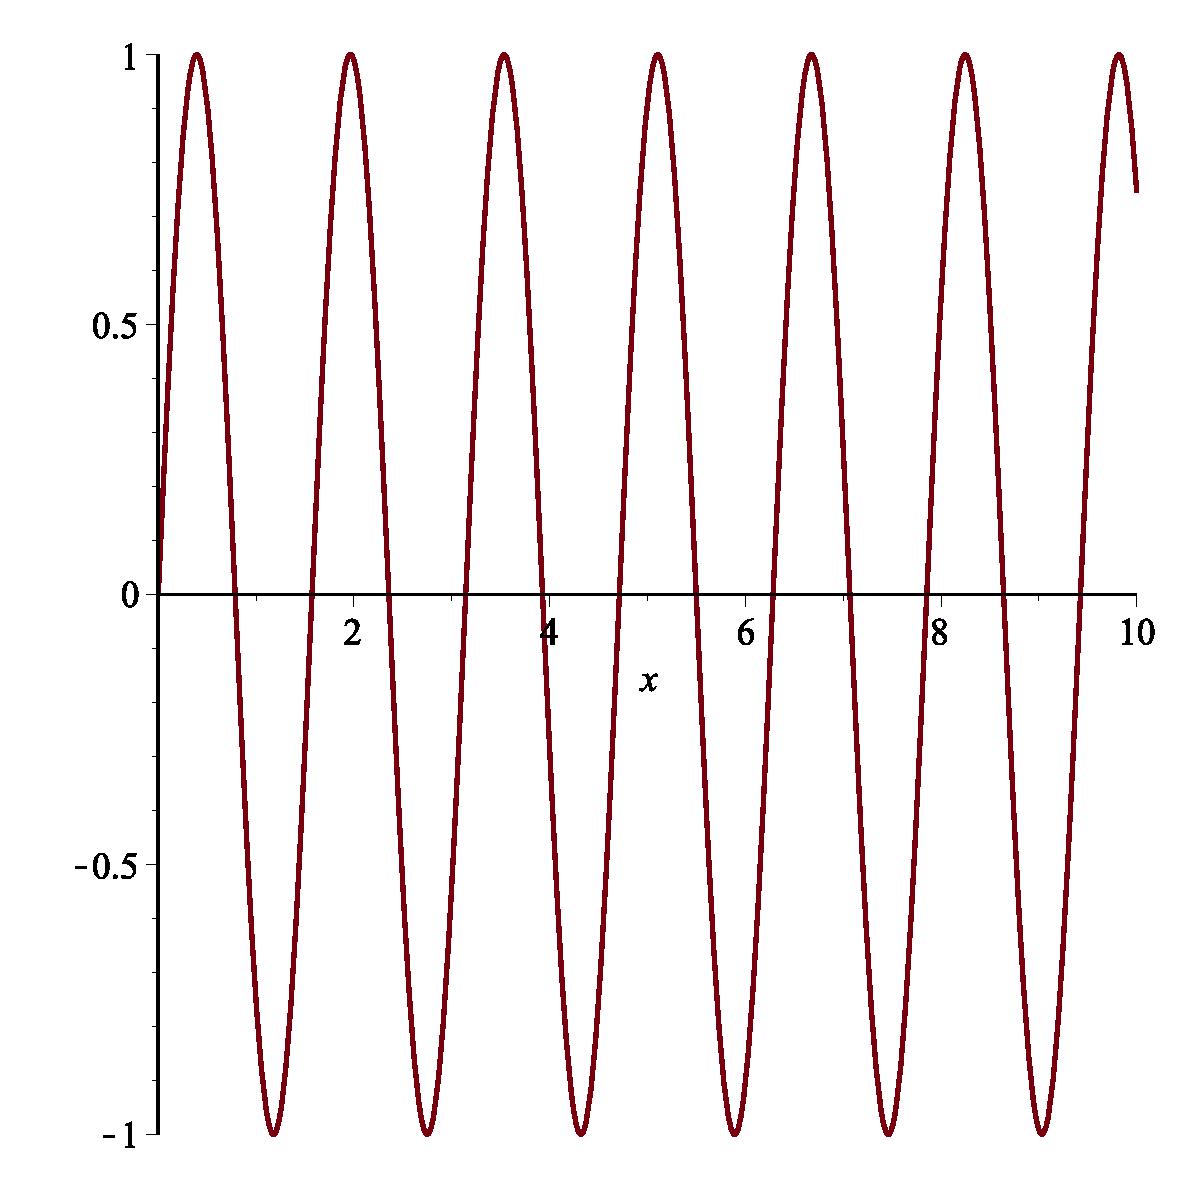
\includegraphics{figures/8_1_Exercise_1.eps}}
\caption{The graph of $f(x) = \sin(4x)$ on the interval $[0,10]$}
\label{F:8.1.PA1}
\end{center}
\end{figure}
We approximate $f$ by \emph{sampling}, that is by partitioning the interval $[0,10]$ into uniform subintervals and recording the values of $f$ at the endpoints.
    \ba
	\item Ineffective sampling can lead to several problems in reproducing the original signal. As an example, partition the interval $[0,10]$ into 8 equal length subintervals and create a list of points (the \emph{sample}) using the endpoints of each subinterval. Plot your sample on graph of $f$ in Figure Figure \ref{F:8.1.PA1}. What can you say about the period of your sample as compared to the period of the original function?

    \item The sampling rate is the number of samples of a signal taken per second. As part (a) illustrates, sampling at too small a rate can cause serious problems with reproducing the original signal (this problem of inefficient sampling leading to an inaccurate approximation is called \emph{aliasing}). There is an elegant  theorem called the Nyquist-Shannon Sampling Theorem that says that human perception is limited, which allows that replacement of a continuous signal with a digital one without any perceived loss of information. This theorem also provides the \emph{lowest} rate at which a signal can be sampled (called the Nyquist rate) without such a loss of information. The theorem states that we should sample at double the maximum desired frequency so that every cycle of the original signal will be sampled at at least two points.

        Recall that the frequency of a sinusoidal function is the reciprocal of the period. Identify the frequency of the function $f$ and determine the number of partitions of the interval $[0,10]$ that give us the Nyquist rate.

    \item Humans cannot typically pick up signals above 20 kHz. Explain why, then, that information on a compact disk is sampled at 44,100 Hz.


    \ea


\end{exercises}
\afterexercises
